\chapter{\textbf{Рассчётный магнитный момент в различных кластерах}}\label{ch:results}
С помощью метода рассеянных волн расчитаны кривые зависимости плотности состояний электронов от энергии, а также
зависимости полной и спиновой плотностей электронов от расстояния до ядра. Таким образом показано, что в этих кластерах
возникают магнитные свойства (такой же вывод даёт эксперимент).

\section{\textbf{Al4C6}}\label{sec:results/al4c6}
Обособленный атом углерода обладает магнитным моментом, поскольку оболочки в нём незаполнены. Когда углерод
входит в химическое соединение, его оболочки заполняются и магнитный момент пропадает "---так происходит обыкновенно.
Однако, нами было показано, что в кластере определённой геометрии (рисунок \cref{fig:al4c6}), когда атомы углерода разделены
атомами алюминия, магнитный момент сохраняется.

\begin{figure}[ht]
  \centerfloat{
    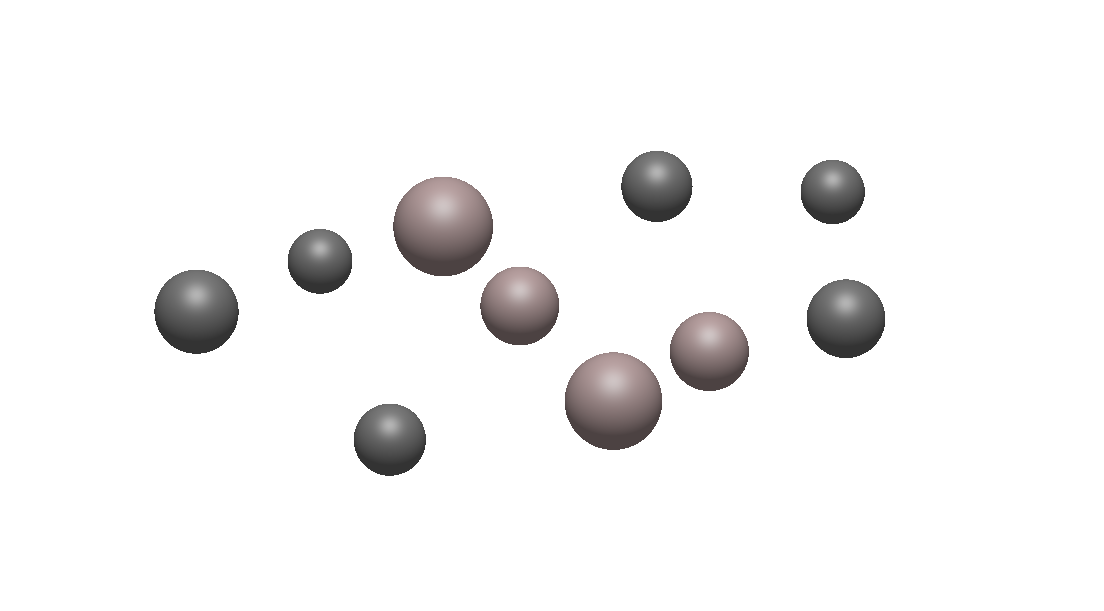
\includegraphics[scale=0.5]{al4c6}
  }
  \caption{Изображение кластера Al4C6, построенное с помощью программы Avogadro 1.93.0\cite{Hanwell2012}}
  \label{fig:al4c6}
\end{figure}

Из кривой плотности состояний (рисунок \cref{fig:al4c6-spectrum})видно, что электроны с разным спином распределяются по
оболочкам неравномерно, как следствие возникает магнитный момент, в среднем на атом равный 0.58 магнетона Бора.
\begin{figure}[ht]
  \centerfloat{
    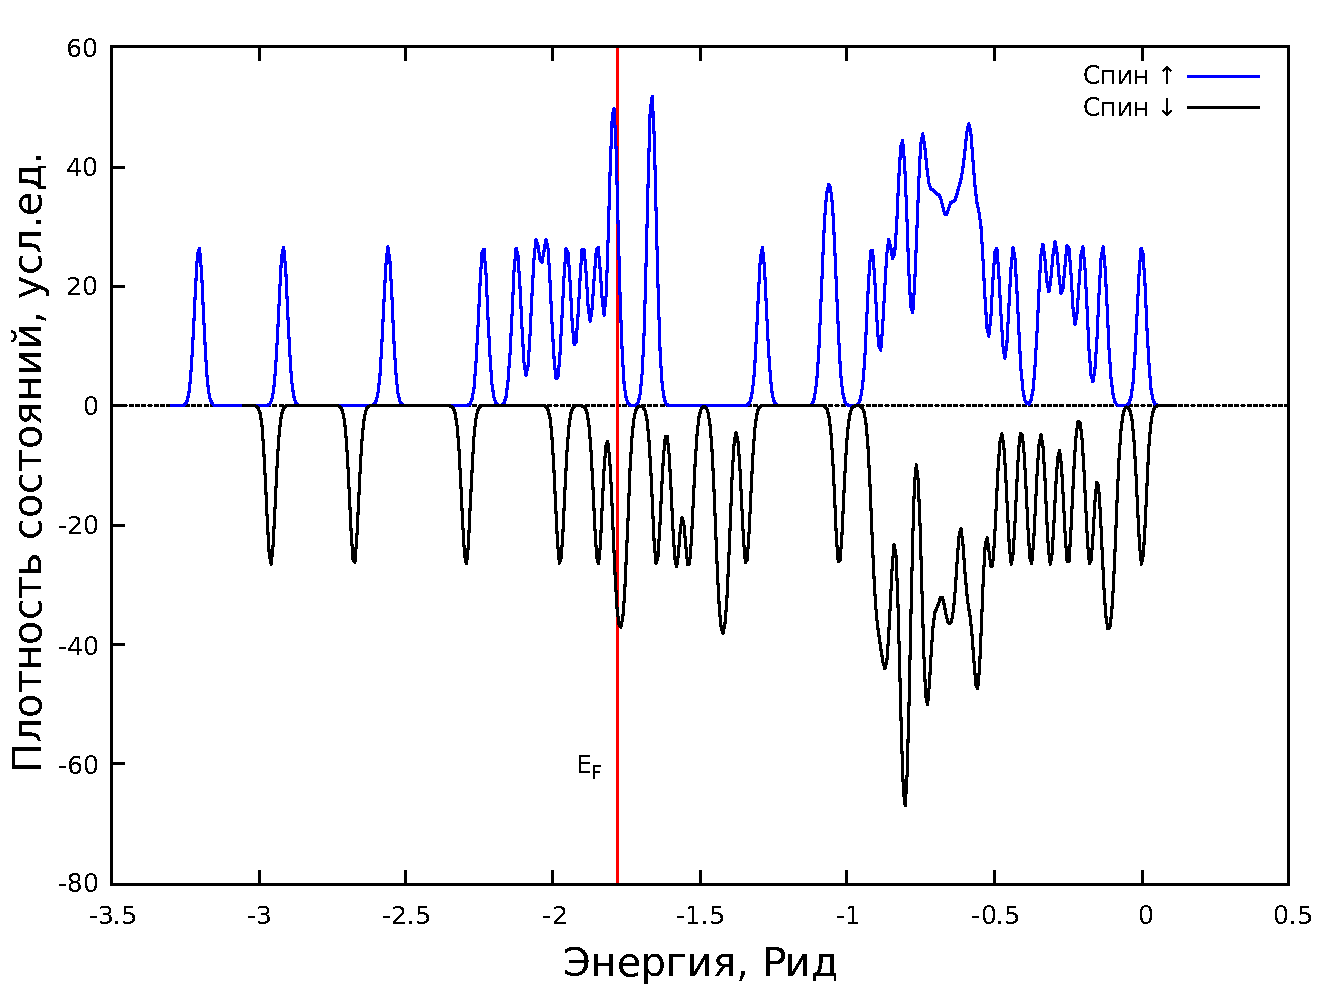
\includegraphics[scale=0.5]{al4c6-spectrum}
  }
  \caption{Зависимость плотности состояний электронов от энергии для кластера Al4C6}
  \label{fig:al4c6-spectrum}
\end{figure}

\section{\textbf{Ti6Ni4}}\label{sec:results/ti6ni4}
Такая же кривая плотности состояний была просчитана для кластера Ti6Ni4 (рисунок \cref{fig:ti6ni4-spectrum}). Расчётный
средний магнитный момент на атом составил 0.24 магнетона Бора.
\begin{figure}[ht]
  \centerfloat{
    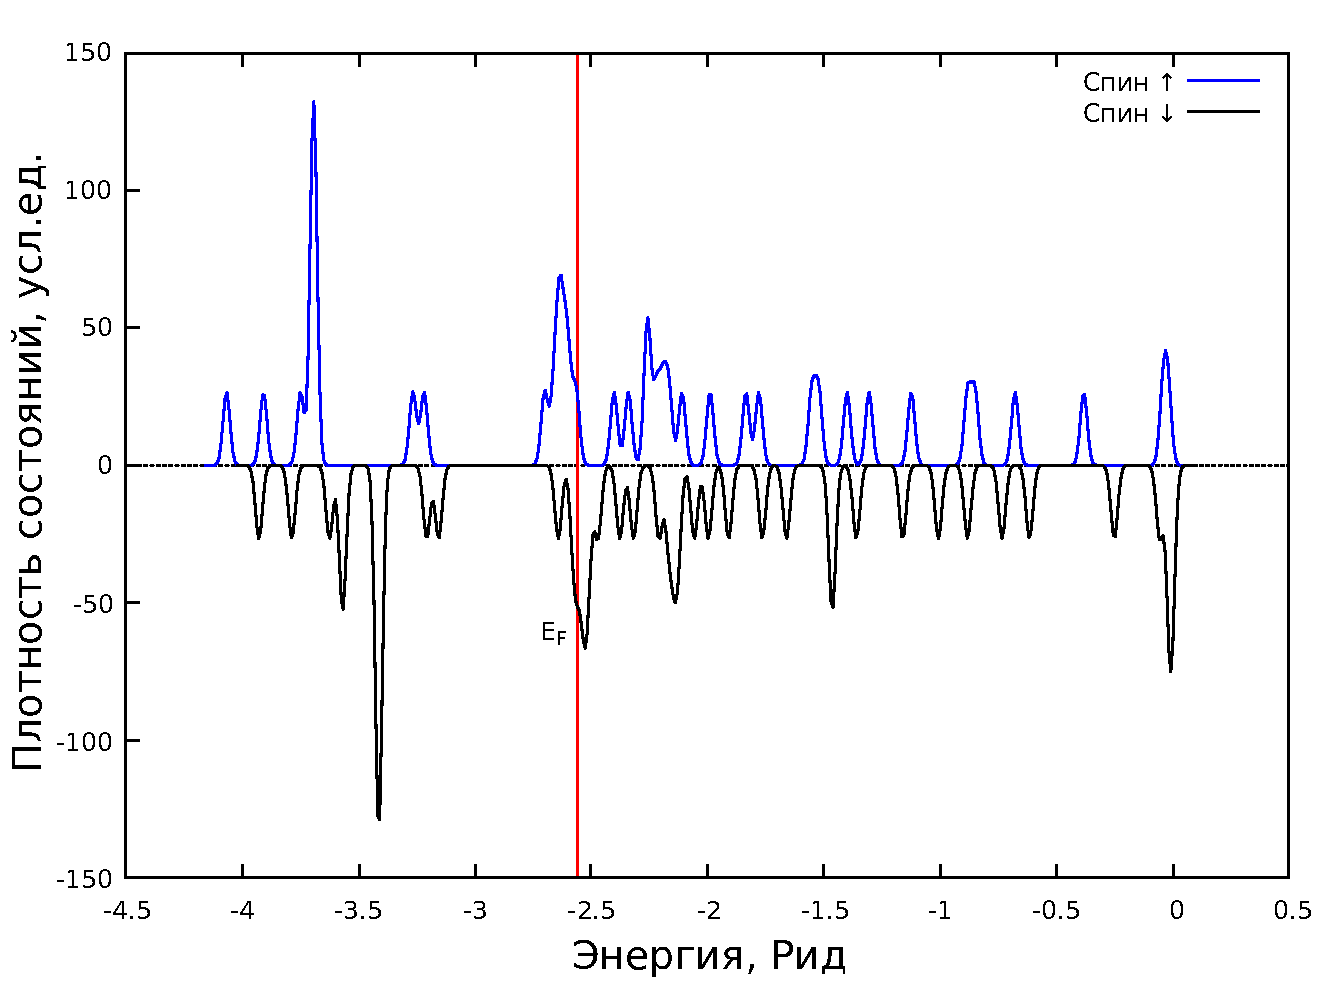
\includegraphics[scale=0.5]{ti6ni4-spectrum}
  }
  \caption{Зависимость плотности состояний электронов от энергии для кластера Ti6Ni4}
  \label{fig:ti6ni4-spectrum}
\end{figure}

\section{\textbf{Fe10}}\label{sec:results/fe10}
Интересным направлением является исследование магнитного момента у кластеров железа в зависимости от числа входящих
в них атомов. Для кластера железа спиралевидной формы, состоящего из десяти атомов, средний магнитный момент
на атом составил 0.26 магнетона Бора, соответствующая кривая плотности состояний приведена на
рисунке~\cref{fig:fe10-spectrum}.
\begin{figure}[ht]
  \centerfloat{
    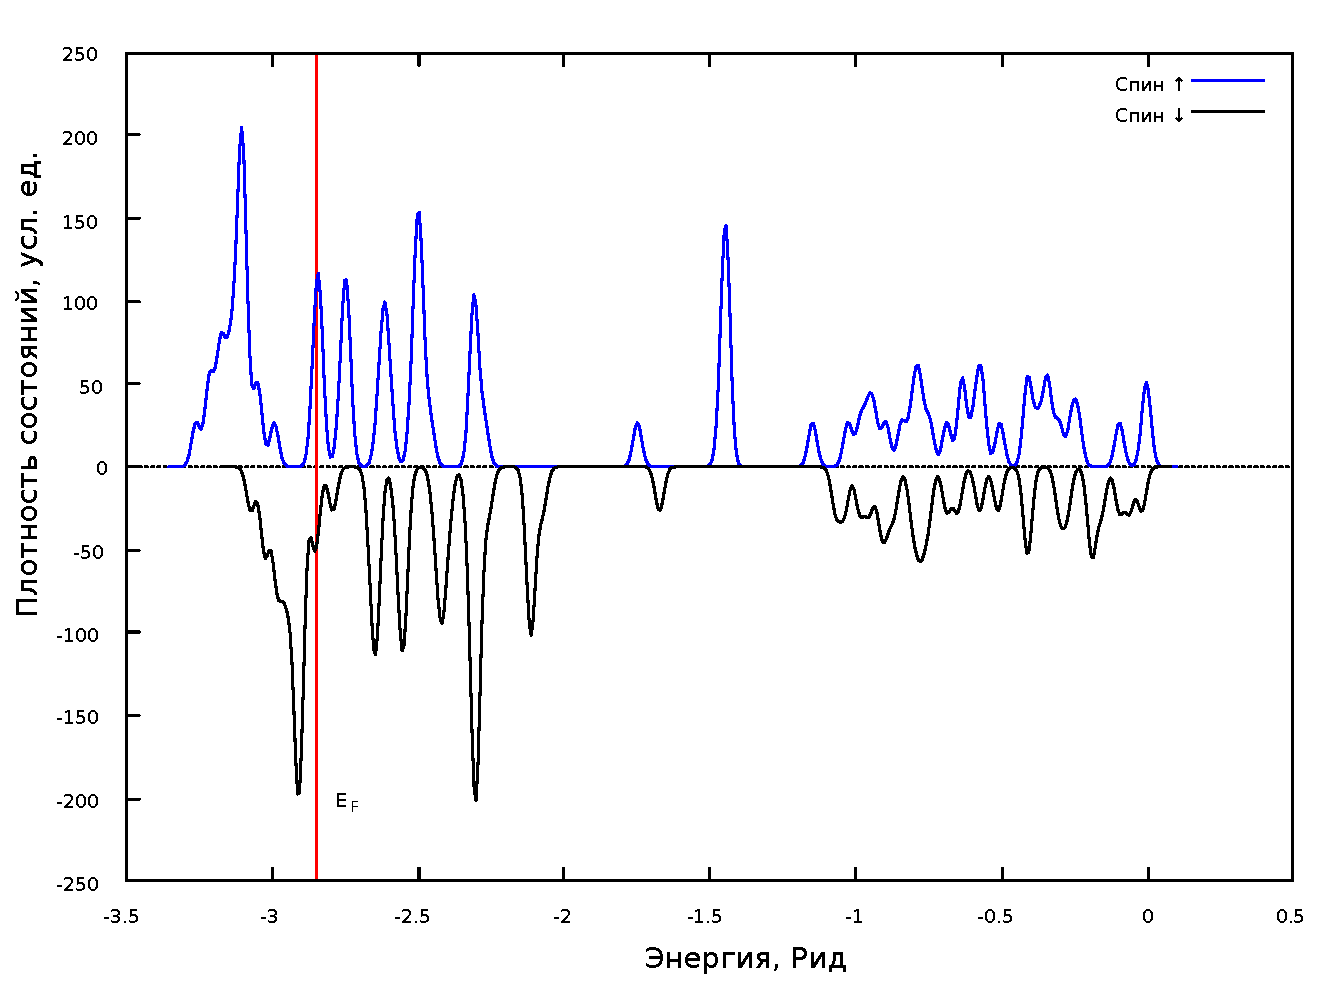
\includegraphics[scale=0.5]{fe10-spectrum}
  }
  \caption{Зависимость плотности состояний электронов от энергии для кластера Fe10}
  \label{fig:fe10-spectrum}
\end{figure}

\section{\textbf{Fe12}}\label{sec:results/fe12}
Для кластера железа такой же спиральной формы, но из двенадцати атомов, а не десяти, средний магнитный момент на атом
составил 0.21 магнетона Бора, кривая плотности приведена на рисунке~\cref{fig:fe12-spectrum}. Также для атома железа
в данном кластере приведём график зависимости полной плотности электронов от расстояния до ядра атома
(рисунок~\cref{fig:fe12-full}) и спиновой плотности электронов от расстояния до ядра атома
(рисунок~\cref{fig:fe12-spin-3}). На рисунке~\cref{fig:fe12-spin-1} изображена та же спиновая плотность электронов,
но в большем масштабе, так, чтобы было видно поведение кривой при малых $r$.
\begin{figure}[ht]
  \centerfloat{
    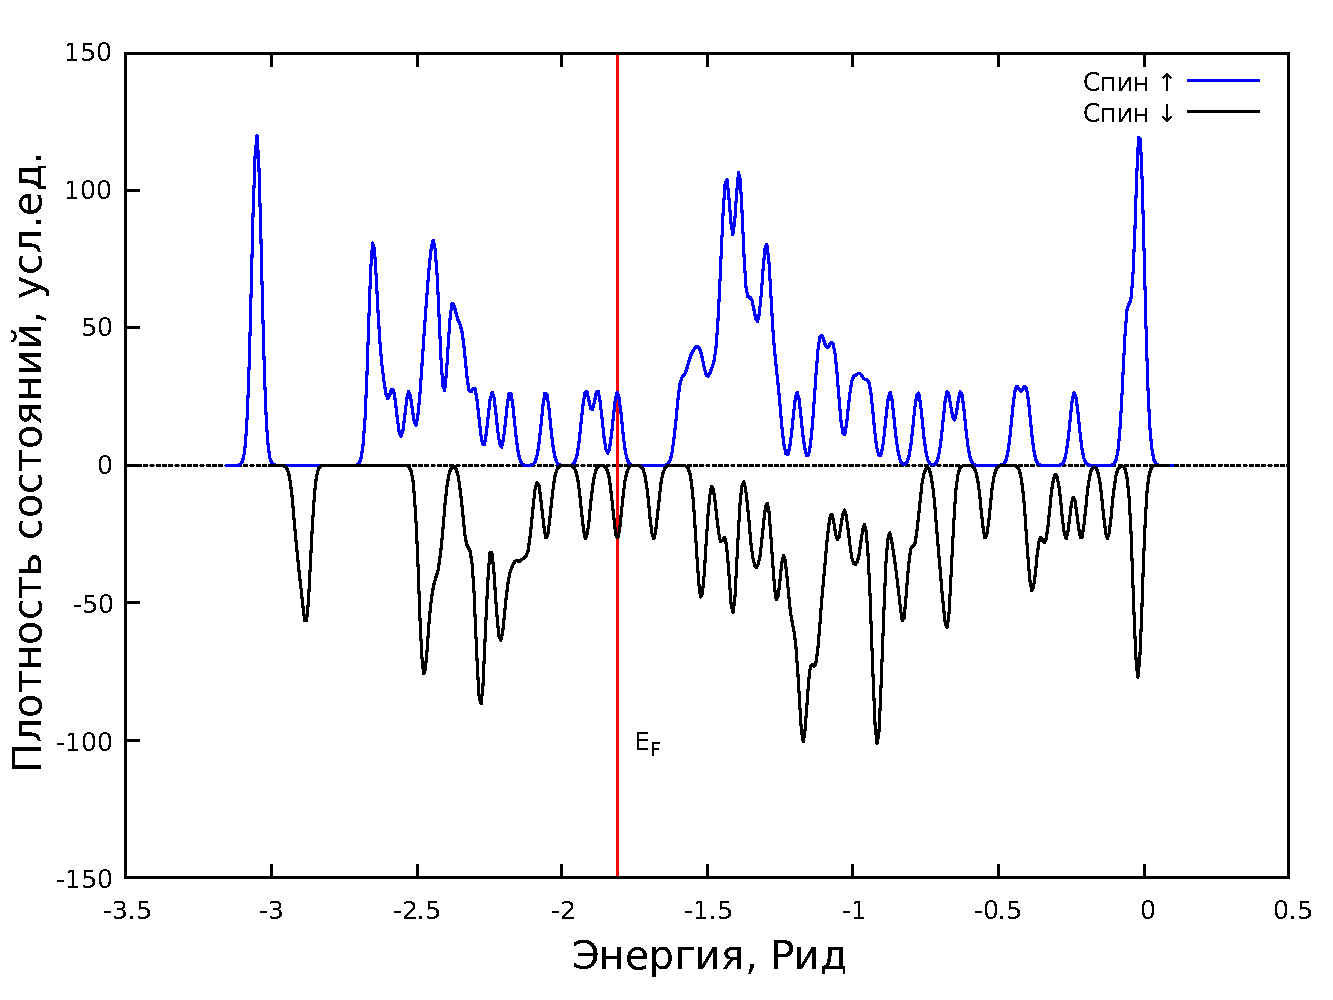
\includegraphics[scale=0.5]{fe12-spectrum}
  }
  \caption{Зависимость плотности состояний электронов от энергии для кластера Fe12}
  \label{fig:fe12-spectrum}
\end{figure}

\begin{figure}[ht]
  \centerfloat{
    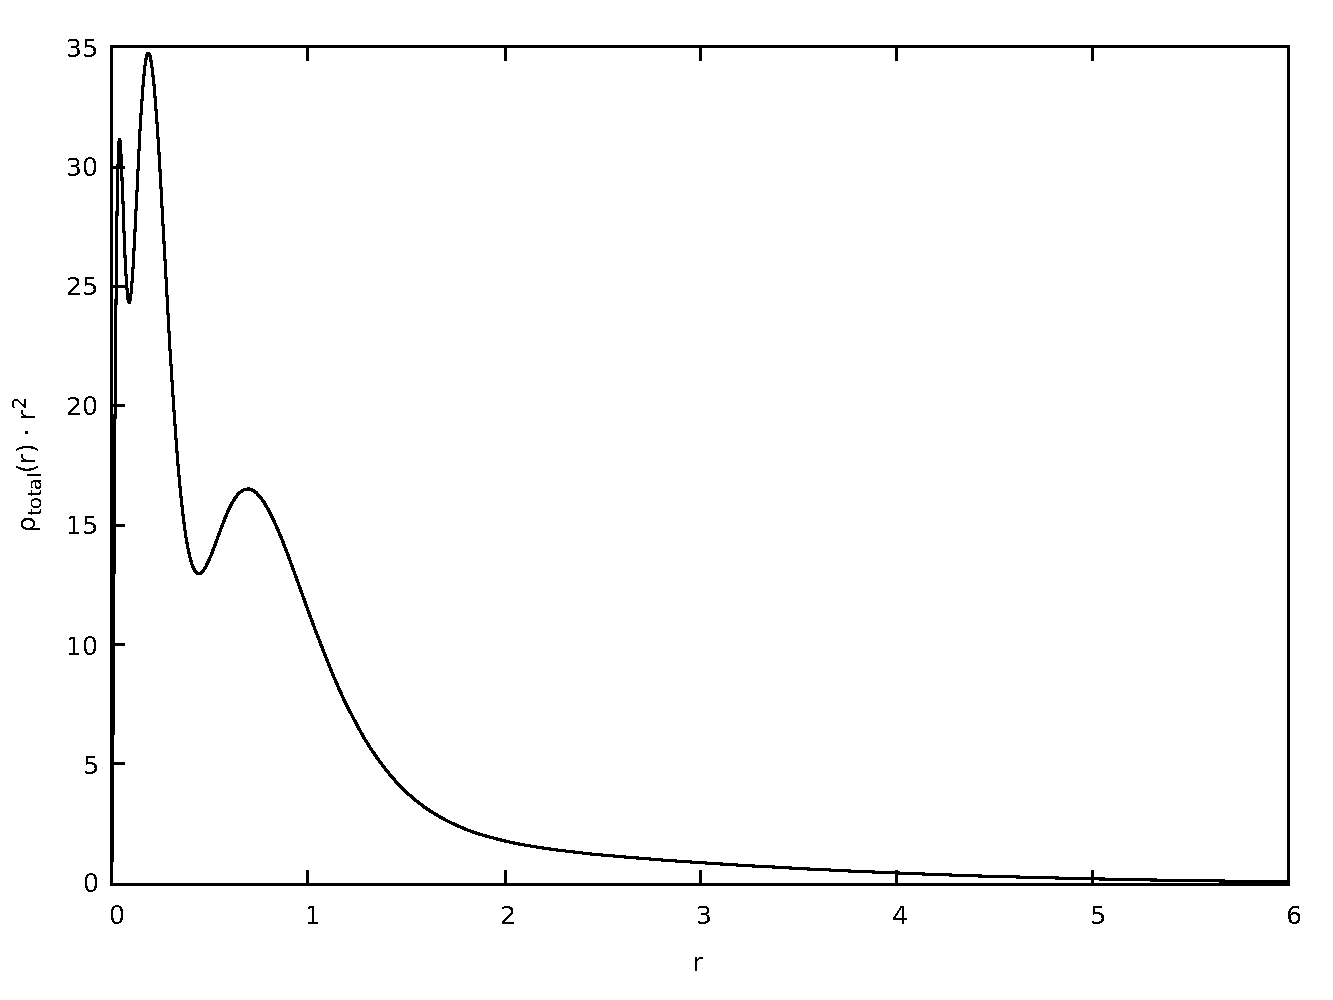
\includegraphics[scale=0.5]{fe12-full}
  }
  \caption{Зависимость полной плотности электронов от расстояния до ядра у атома железа в кластере Fe12}
  \label{fig:fe12-full}
\end{figure}

\begin{figure}[ht]
  \centerfloat{
    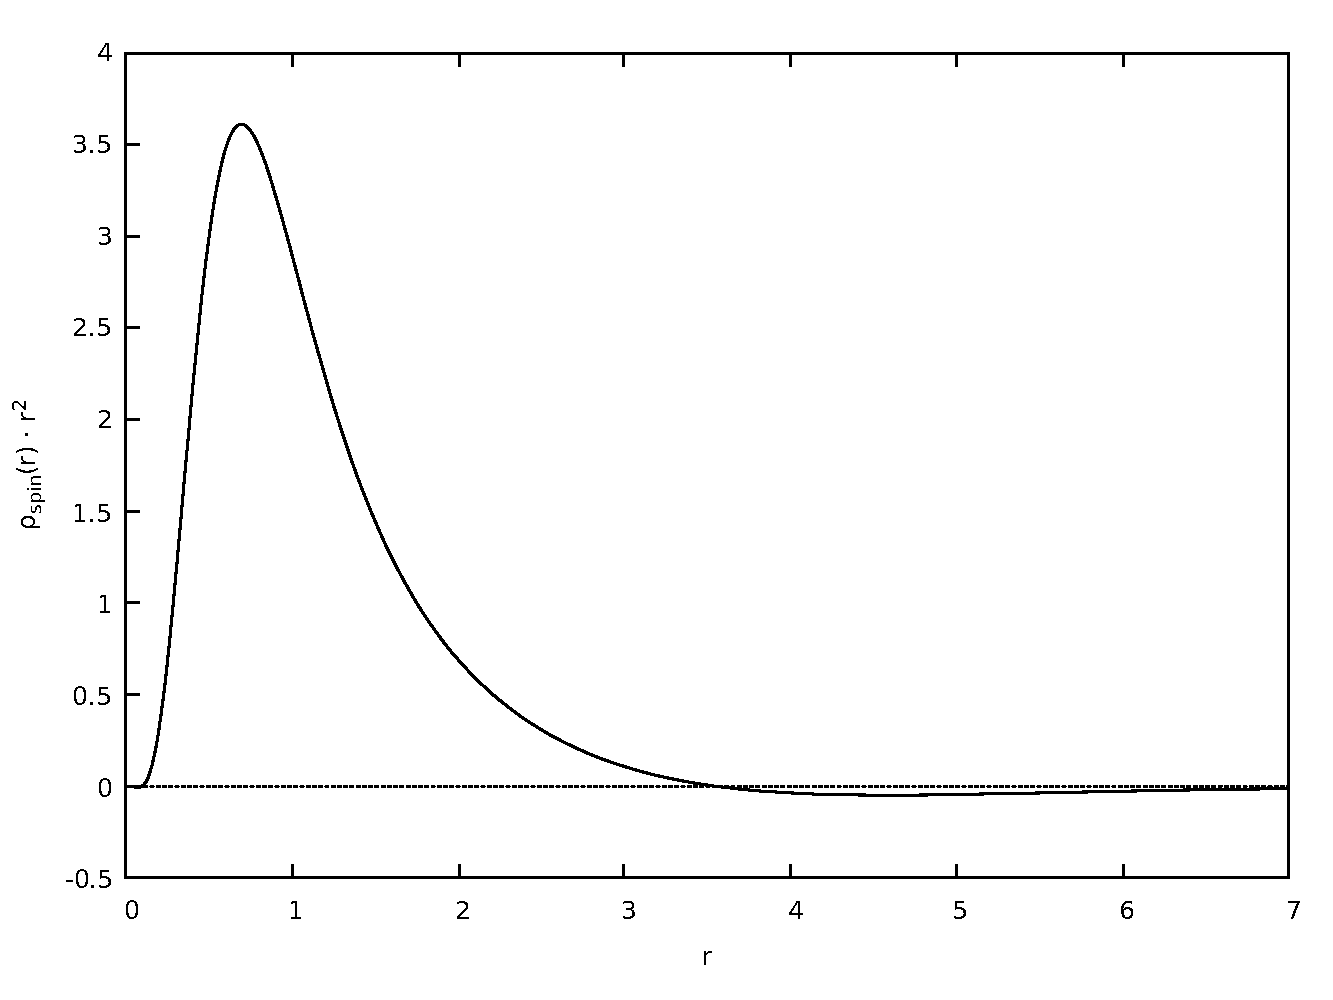
\includegraphics[scale=0.5]{fe12-spin-3}
  }
  \caption{Зависимость спиновой плотности электронов от расстояния до ядра у атома железа в кластере Fe12}
  \label{fig:fe12-spin-3}
\end{figure}

\begin{figure}[ht]
  \centerfloat{
    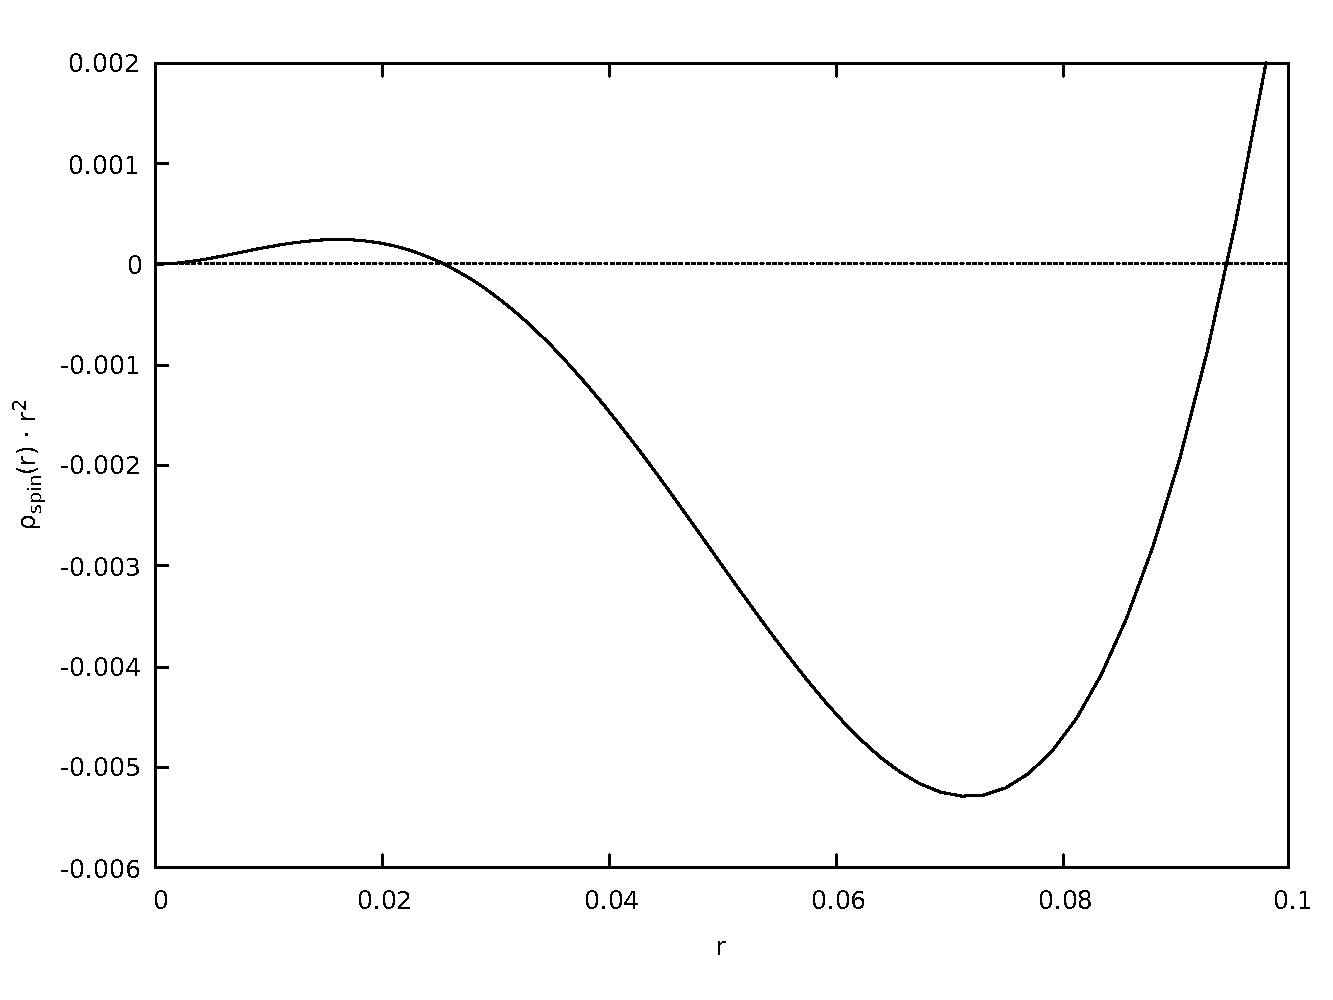
\includegraphics[scale=0.5]{fe12-spin-1}
  }
  \caption{Зависимость спиновой плотности электронов от расстояния до ядра у атома железа в кластере Fe12 в большем масштабе}
  \label{fig:fe12-spin-1}
\end{figure}

\FloatBarrier
